\documentclass{beamer}

\usepackage{graphicx,hyperref,udesc,url}
\usepackage[latin1]{inputenc}
%\usepackage[T1]{fontenc}
\usepackage{booktabs}
\usepackage[portuges]{babel}


\title[On Understanding Types, Data Abstraction and Polymorphism]{On Understanding Types, Data Abstraction\\ and Polymorphism}

\author[Rafael Castro]{
    Rafael Castro G. Silva\\\medskip
    {\small \url{rafaelcgs10@gmail.com}}
    }

    \institute[UDESC]{
        Departamento de Ci\^encia da Computa\c{c}\~ao \\
            Centro de Ci\^encias e Tecnol\'ogicas\\
            Universidade do Estado de Santa Catarina}

\begin{document}

\begin{frame}
\titlepage

\end{frame}

\section{Classifica��o de sistemas de tipos}
\begin{frame}[plain]
\frametitle{Classifica��o de Sistemas de Tipos}
    \begin{figure}
        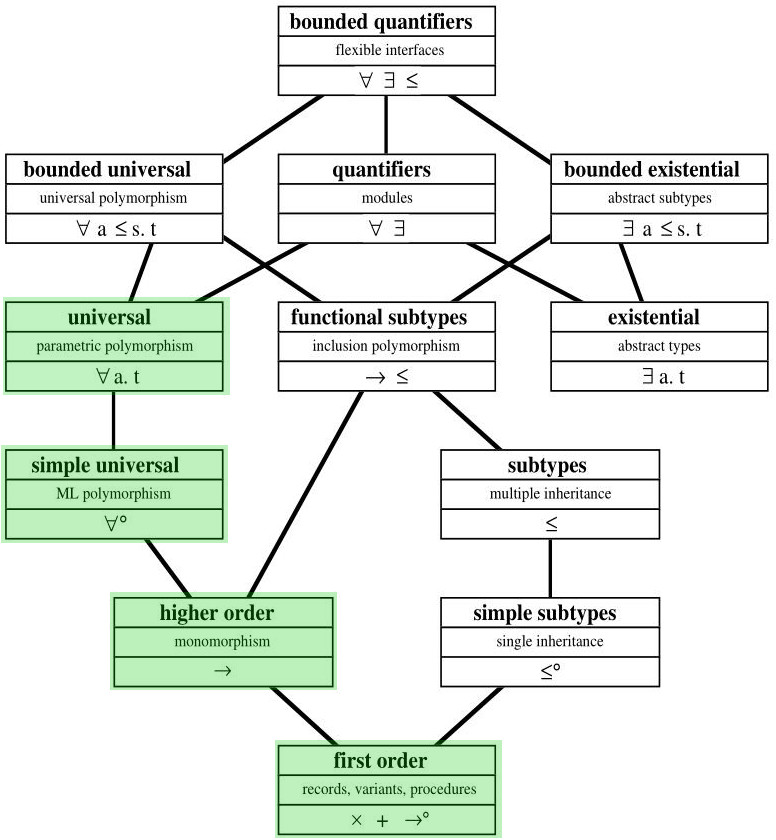
\includegraphics[width = 0.65\textwidth]{typesystems.jpeg}
      \caption{Classifica��o Sistemas de Tipos. Retirado de [1].}
  \centering
    \end{figure}
\end{frame}

\section{Sistemas de tipos monom�rficos}
\begin{frame}
\frametitle{Primeira Ordem}
    \begin{align*}
      FunType & := ConstType \rightarrow FunType \\
      ConstType & := Int, Float, String...
    \end{align*}
  \begin{itemize}
    \item Fun��es n�o s�o dados.
    \item Linguagens: Java $<$ 8, Python $<$ 2, Ruby...
  \end{itemize}
\end{frame}

\begin{frame}
\frametitle{Ordem Superior}
    \begin{align*}
      Type & := Type \rightarrow Type | ConstType\\
      ConstType & := Int, Float, String...
    \end{align*}
  \begin{itemize}
    \item Fun��es s�o dados.
    \item Linguagens: Algol 68, Fortran, C, Pascal, Java $\geq$ 8, Python $\geq$ 2, Haskell...
  \end{itemize}
\end{frame}

\section{Sistemas de tipos polim�rficos}
\begin{frame}
  \frametitle{Polimorfismo ML (Simple Universal)}
    \begin{align*}
      PolyType & := \forall VarType . PolyType | Type \\
      Type & := Type \rightarrow Type | ConstType | VarType\\
      ConstType & := Int, Float, String...\\
      VarType & := a, b, c...
    \end{align*}
  \begin{itemize}
    \item Fun��es s�o polim�rficas: uma fun��o assume v�rios tipos.
    \item Fun��es de ordem superior tratam argumentos de maneira monom�rfica.
    \item Linguagens: ML, OCaml, Haskell...
  \end{itemize}
\end{frame}

\begin{frame}
  \frametitle{Segunda Ordem (Universal)}
    \begin{align*}
      Poly & := \forall VarType . Type | Type \rightarrow Type | ConstType | VarType\\
      ConstType & := Int, Float, String...\\
      VarType & := a, b, c...
    \end{align*}
  \begin{itemize}
    \item Fun��es s�o polim�rficas: uma fun��o assume v�rios tipos.
    \item Fun��es de ordem superior tratam argumentos de maneira polim�rficas.
    \item Linguagens: Haskell...
  \end{itemize}
\end{frame}


\begin{frame}
  \frametitle{Refer�ncias}
  [1] On Understanding Types, Data Abstraction and Polymorphism, Luca Cardelli and Peter Wegner.
\end{frame}
\end{document}
